\documentclass[10pt]{article}
\usepackage{graphicx} % Required for including images
\usepackage[T1]{fontenc} % Use 8-bit encoding that has 256 glyphs
\usepackage[utf8]{inputenc} % Required for including letters with accents
\usepackage{amsmath,amssymb,amsthm} % For including math equations, theorems, symbols, etc
\usepackage{quotes} % for quotation marks

\title{Projektskizze}

\begin{document}

\begin{titlepage}

\raggedleft % Right align everything
	
	\vspace*{\baselineskip} % Whitespace at the top of the page
	
	\rightline{{\large Claudio Frei, Karin Birle, Leo Rudin,}} 
	\rightline{\large Michael Wigger, Nathalie Achtnich, Philippe Schneider,} 
	\rightline{\large Raphael Krebs, Silvan Nigg, Stefan Enz}
	
	\vspace*{0.167\textheight} % Whitespace before the title
	
	\textbf{\LARGE Virtual CT Board}\\[\baselineskip] % First title line
	
	\Huge Projektskizze\\[\baselineskip] % Main title line 
	
	\vfill % Whitespace 
	
	{\large ZHAW - FS 2022}
	
	\vspace*{3\baselineskip} % Whitespace at the bottom of the page


\end{titlepage}

\tableofcontents

\newpage 

\section{Ausgangslage}

Jedes Jahr beginnen fast 200 Studentinnen und Studenten ein Bachelorstudium der Informatik an der ZHAW. Zu ihren Pflichtmodulen in den ersten Jahren gehört die Veranstaltung "Computertechnik 1", die die grundlegende Funktionsweise eines Computers an der Schnittstelle zwischen Hardware und Software behandelt. Im dazugehörigen Praktikum probieren die Studenten das erworbene Wissen selbst aus und benutzen dabei als Hardware ein sogenanntes CT Board, das über einen Prozessor und einen Speicher verfügt und diverse Input-/Output-Möglichkeiten bereitstellt (siehe Abbildung \ref{ctboard}). Damit sie die Übungen auch zuhause durchführen können, leihen die Studenten zu Beginn des Semesters ein solches CT Board von den Dozenten aus. Dieses muss von ihnen nach Hause transportiert und am Ende des Jahres wieder zurückgebracht werden.

\begin{figure}[h]
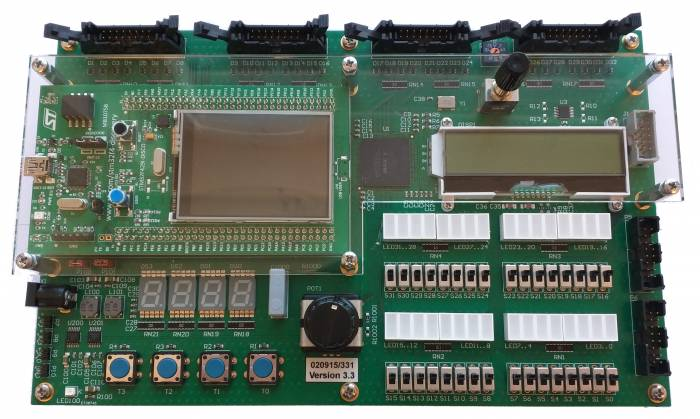
\includegraphics[width=\textwidth]{ctboard}
\caption{Das CT Board, das den Studenten im Modul Computertechnik 1 als Hardware zur Verfügung gestellt wird. (Quelle: ennis.zhaw.ch)}
\label{ctboard}
\end{figure}

\section{Idee}

Im 21. Jahrhundert noch Hardware an Studenten zu verleihen, mutet schon fast archaisch an. Insbesondere, wenn sich die Hardware leicht als Software simulieren liesse. Und genau hier setzt unsere Idee an: Wir möchten eine Web-Applikation entwickeln, die ein CT Board simuliert und von den Studenten anstelle dessen für die "Computertechnik 1"-Praktika eingesetzt werden kann. Die Studenten können die Übungen mit unserem leichtgewichtigen "Virtual CT Board" genauso gut wie mit dem echten Board lösen und brauchen dafür fortan keine Hardware mehr. Die ZHAW kann sich somit die Beschaffung und Wartung von CT Boards sparen.

\section{Kundennutzen}

Unsere Kundschaft besteht aus zwei Zielgruppen, nämlich die Informatikstudenten der ZHAW auf der einen Seite und die ZHAW als Institution auf der anderen Seite. Für beide Gruppen ergeben sich durch unser Produkt unmittelbare Vorteile:

\paragraph{Für die Studenten:}
\begin{itemize}
\item Die Studenten des Moduls "Computertechnik 1" haben eine elegante Alternative zu den physischen CT Boards und müssen jene nicht mehr nach Hause tragen.
\item Im Gegensatz zum bisherigen physischen CT Board benötigt unser "Virtual CT Board" keinen Strom und lässt sich daher überall - also beispielsweise auch unterwegs - direkt auf dem Laptop starten.
\item Die bisher für den C- und Assembler-Code eingesetzte Software Keil wird überflüssig und muss nicht mehr händisch konfiguriert werden.
\item Es ergeben sich keine Unklarheiten mehr, wie das CT Board mit dem eigenen Computer verkabelt und von diesem aus bedient werden muss.
\item Die Studenten müssen sich nicht mehr darum sorgen, dass ihr geliehenes CT Board kaputtgehen könnte.
\end{itemize}

\paragraph{Für die ZHAW:}
\begin{itemize}
\item Die Lizenz für unsere Software ist um einiges preiswerter als die Beschaffung physischer CT Boards. Die ZHAW spart also Geld.
\item Alte oder defekte Geräte müssen nicht mehr ausgetauscht oder repariert werden. Auch dies spart Geld und Zeit.
\item Die Dozenten müssen für die Praktika nicht mehr mühsam Keil-Projekte konfigurieren. Es genügt, die Assembler-Files ins "Virtual CT Board" hochzuladen.
\end{itemize}

\section{Stand der Technik / Konkurrenzanalyse}

Es existieren bereits verschiedene Produkte, die den Studenten des Moduls "Computertechnik 1" beim Erlernen ihrer Fertigkeiten behilflich sein können. Zum einen gibt es virtuelle Emulatoren für die Assembly-Sprache wie zum Beispiel VisUAL, zum anderen treten wir mit unserem Produkt natürlich auch gegen das physische CT Board an, das aktuell noch in den "Computertechnik"-Praktika verwendet wird.

\paragraph{VisUAL Emulator}
Der Emulator VisUAL von Alman Sarif wurde ebenfalls für ein Einführungsmodul in die Computerarchitektur entwickelt, allerdings am Imperial College in London. Die Software ermöglicht das Schreiben von Assembly-Code in einem Editor-Fenster, der dann via Button ausgeführt wird und dessen Auswirkungen auf die Register und Flags rechts davon angezeigt werden (siehe Abbildung \ref{emulator}).
\begin{figure}[h]
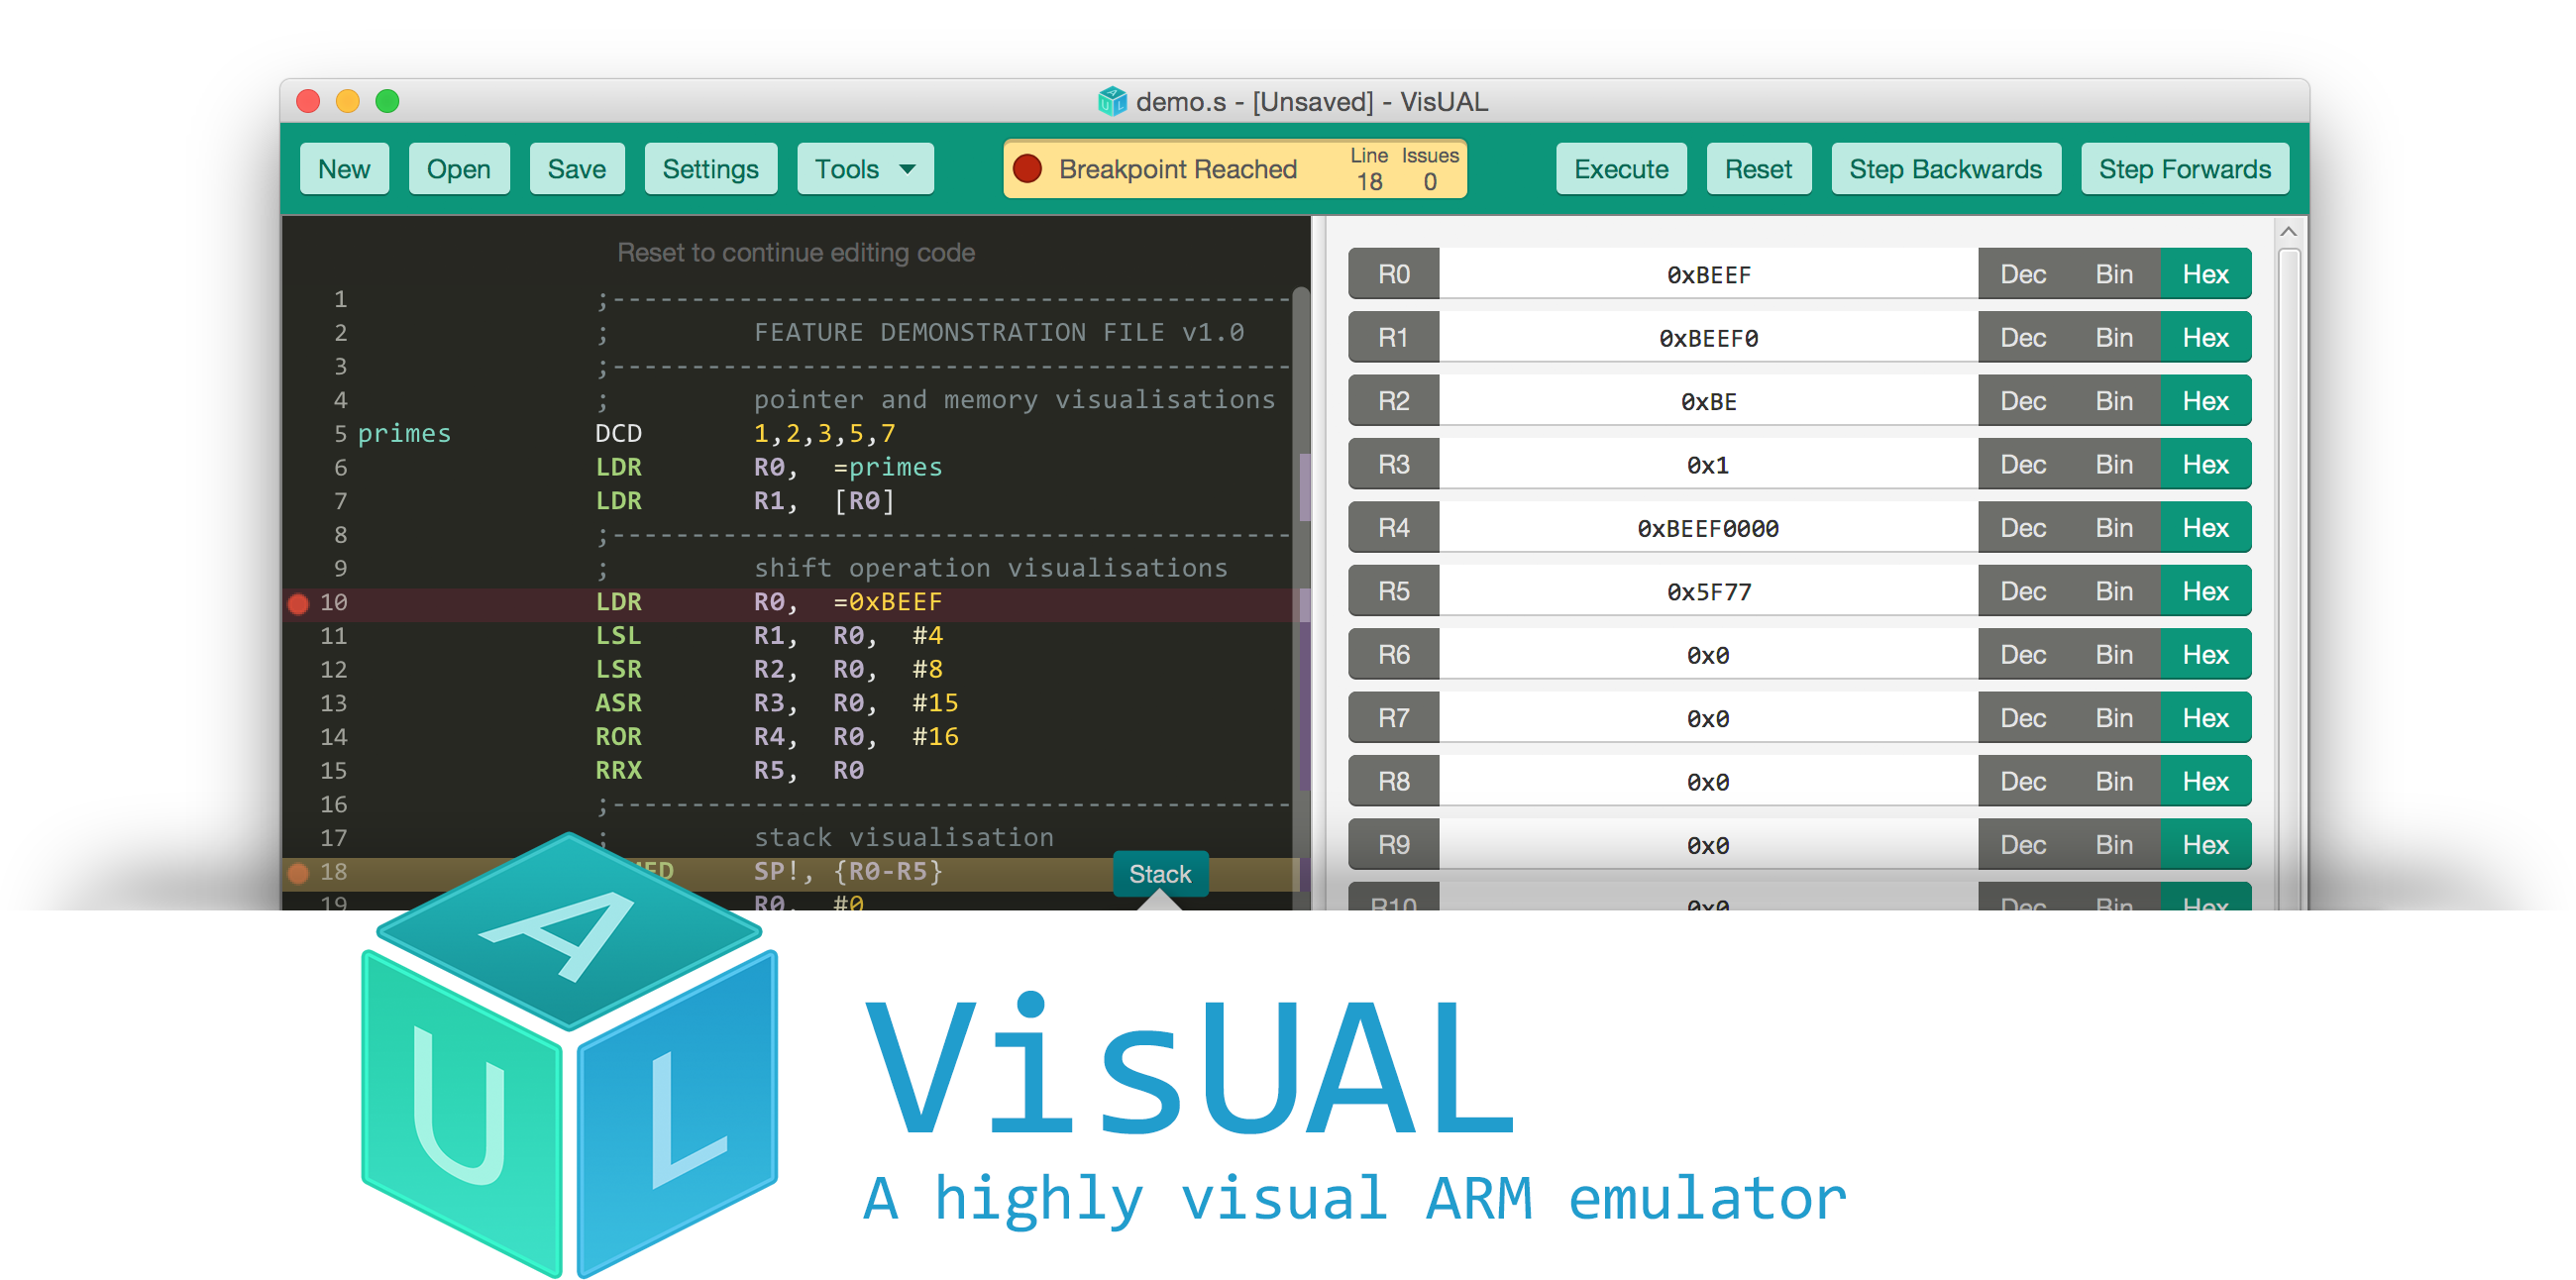
\includegraphics[width=\textwidth]{visual_emulator}
\caption{Der Emulator VisUAL samt seiner grafischen Oberfläche. (Quelle: https://salmanarif.bitbucket.io/visual/index.html)}
\label{emulator}
\end{figure}
Der Unterschied zu unserem "Virtual CT Board" besteht darin, dass VisUAL und auch andere Emulatoren für Assembler nicht auf das CT Board ausgerichtet sind, das die "Computertechnik 1"-Praktika verlangen. Es gibt bei diesen Programmen keine Visualisierung von Hardware-Bestandteilen, mit Ausnahme der Register und Flags. Das bedeutet, dass diese Emulatoren nützlich sind, um in Assembler zu programmieren, jedoch nicht für die Durchführung der "Computertechnik 1"-Praktika an der ZHAW ausreichen. Das "Virtual CT Board" füllt diese Lücke, indem das komplette physische CT Board virtuell visualisiert wird und dieselben Input-/Output-Möglichkeiten bestehen wie beim realen.

\paragraph{physisches CT Board} 

Das physische CT Board soll hier noch einmal erwähnt werden, da es die Hauptkonkurrenz zu unserem Produkt darstellt. Es erfüllt die funktionalen Anforderungen der "Computertechnik 1"-Praktika vollumfänglich und ist ausserdem im Schulbetrieb bereits etabliert. Seine Nachteile bestehen insbesondere in seiner Unhandlichkeit. Das "Virtual CT Board" soll diesen Nachteil genau durch seine Virtualität beheben (siehe dazu Abschnitt "Kundennutzen") und gleichzeitig dem realen CT Board bzgl. Funktionalität in nichts nachstehen. 

\section{Kontextszenario (Hauptablauf)}

Informatikstudentin Anna mag systemnahes Programmieren und hat sich deshalb sehr auf das Modul "Computertechnik 1" gefreut. An den Praktika arbeitet sie am liebsten in Ruhe zuhause. Dafür öffnet sie das "Virtual CT Board" im Browser und lädt den vorgegebenen Coderahmen im Programm hoch. In der Praktikumsanleitung liest sie nach, was zu tun ist. Der vorgegebene Programmcode ist im integrierten Texteditor im Browser sichtbar, den sie jetzt um verschiedene Assembler-Befehle erweitert. Als sie auf den "Run"-Button klickt, wird das Assembly-Programm ausgeführt und auf das virtuelle CT Board "geladen", das ganz rechts im Browser ersichtlich ist. 
\newline Auf diesem virtuellen CT Board klickt Anna nun auf einige der DIP Switches, doch es passiert nichts. Anna führt den Code nochmals im Debug-Modus Schritt für Schritt aus und kontrolliert dabei jeweils die Registerinhalte, die in der Mitte des Browsers angezeigt werden. Da bemerkt sie einen semantischen Fehler, den sie schnell korrigiert. Sie lässt den Code nochmals im normalen Modus laufen und klickt wieder die kleinen Schalter an - diesmal beginnen die dazugehörigen LED-Lämpchen zu leuchten. Sie ist zufrieden, weil das Programm nun so funktioniert, wie es gemäss Anleitung sollte. Also speichert Anna speichert das File ab und gibt das Praktikum in der nächsten Stunde erfolgreich ab.

\section{Weitere Anforderungen}

\section{Ressourcen}

\section{Risiken}

\section{Wirtschaftlichkeit}

\end{document}